\documentclass[11pt,oneside]{article}
\usepackage[letterpaper,margin=1in]{geometry}
\usepackage[T1]{fontenc}
\usepackage{lmodern,microtype}
\usepackage{booktabs,tabularx,array,float}
\usepackage[numbers]{natbib}
\usepackage{pgfplots}
\usepackage{hyperref}
\pgfplotsset{compat=1.18}
\definecolor{inkblue}{HTML}{153B58}
\definecolor{tealplot}{HTML}{087F78}
\hypersetup{colorlinks=true,linkcolor=inkblue,citecolor=inkblue,urlcolor=inkblue,
  pdftitle={CS781 Capstone Project - In-House Legal Intelligence System},
  pdfauthor={Hardik Tiwari}}
\newcolumntype{Y}{>{\raggedright\arraybackslash}X}
\setlength{\parskip}{4pt}
\setlength{\parindent}{0pt}
\raggedbottom

\title{CS781 Capstone Project:\\
In-House Legal Intelligence System}
\author{Hardik Tiwari\\
230437\\
\texttt{hardikt23@iitk.ac.in}\\
Indian Institute of Technology Kanpur (IIT Kanpur)}
\date{}

\begin{document}
\maketitle

\begin{abstract}

This project trains compact models for Indian legal text so the processing can run on infrastructure controlled by the document holder. Four foundations of about 50 million parameters were trained from scratch on Acts and decisions from High Courts, the Supreme Court and tribunals. Their tokenizer and checkpoints support six downstream tasks: entity recognition, rhetorical role labeling, judgment prediction, statute identification, summarization and precedent retrieval. The balanced decoder recorded 0.8302 BERTScore F1 in the pretraining competition. The distilled retriever recorded 0.2593 Micro-F1@7, the highest visible Phase 7 score. The report distinguishes development results from competition scores and identifies summarization as a code deliverable whose completed run has yet to be verified.

\end{abstract}

\section{Competition Result}
\textbf{Source code} \href{https://github.com/hardik4tiwari/cs781-230437}{\texttt{hardik4tiwari/cs781-230437}}

\begin{table}[H]
\centering\small
\caption{Best documented Codabench scores and visible finished rows.}
\begin{tabularx}{\linewidth}{@{}cYlcc@{}}
\toprule
Phase & Task & Primary metric and score & Rank & Finished \\
\midrule
1 & Legal LM pretraining & BERTScore F1 \enspace 0.8302 & --- & 7 \\
2 & Legal named entity recognition & Strict macro-F1 \enspace 0.5061 & --- & 8 \\
3 & Rhetorical role prediction & Macro-F1 \enspace 0.4542 & --- & 7 \\
4 & Court judgment prediction & Macro-F1 \enspace 0.6980 & --- & 7 \\
5 & Legal statute identification & Macro-F1 \enspace 0.3982 & --- & 7 \\
6 & Abstractive summarization & BERTScore F1 \enspace unverified & --- & --- \\
7 & Prior case retrieval & Micro-F1@7 \enspace 0.2593 & --- & 8 \\
\bottomrule
\end{tabularx}
\end{table}

The Phase 1--4 figures come from the earlier project record, while Phases 5 and 7 can be checked against saved Codabench submission views. Together they account for 44 visible finished rows. The records do not establish the Codabench username, distinct valid submission totals, or leaderboard ranks at a common date. The course requires four distinct submissions in Phase 1 and six in each subsequent phase \citep{course}.

\section{Introduction and Problem Description}

A single judgment can contain party names, several statutes, arguments on both sides and citations to earlier decisions. Each downstream task asks a different question of the same text. Entity recognition needs exact offsets, rhetorical role prediction needs sentence order, and retrieval needs a ranking over a separate set of cases. The shared part of this system is the pretrained foundation and tokenizer. The task heads and prediction formats are trained and evaluated separately.

The course required scratch pretraining with official data and a foundation in the 50--300 million parameter range \citep{course}. The experiments compare four similarly sized foundations, then compare full tuning, smaller adaptation modules and distillation where the phase permits them. For long judgments, the workflows use windows, chunk hierarchies, sentence selection or ranked candidates according to the task. Table~\ref{tab:tasks} gives the input and output for each phase.

\begin{table}[H]
\centering\small
\caption{Inputs and outputs of the course tasks.}
\label{tab:tasks}
\begin{tabularx}{\linewidth}{@{}cYY@{}}
\toprule Phase & Input & Output \\ \midrule
1 & 512-word legal prompt & 128-word legal continuation \\
2 & Legal document & Entity types and exact character spans \\
3 & Ordered sentences from a legal document & One rhetorical role per sentence \\
4 & Court judgment text & Binary outcome label \\
5 & Legal document & Set of statute IDs \\
6 & Long legal document & Abstractive summary \\
7 & Query case and candidate pool & Seven ranked candidate case IDs \\
\bottomrule
\end{tabularx}
\end{table}

\section{Data Analysis and Preprocessing}
\subsection{Sources and official splits}

The notebooks use the \texttt{Exploration-Lab/CS-781-Capstone} dataset \citep{course}. In Phase 1, documents are assigned to training or development by hash before packing. Table~\ref{tab:mix} counts tokens in the resulting corpus. The training budget was about 200 million supervised tokens per foundation.

\begin{table}[H]
\centering\small
\caption{Phase 1 corpus mix measured after packing.}
\label{tab:mix}
\begin{tabular}{@{}lrrrr@{}}
\toprule Source & Train tokens & Dev tokens & Train docs & Dev docs \\ \midrule
Acts & 24,000,000 & 200,000 & 2,914 & 37 \\
High Courts & 108,000,000 & 900,000 & 196,540 & 1,591 \\
Supreme Court & 60,000,000 & 500,000 & 12,140 & 88 \\
Tribunals & 48,000,000 & 400,000 & 14,232 & 51 \\
\midrule Total & 240,000,000 & 2,000,000 & 225,826 & 1,767 \\ \bottomrule
\end{tabular}
\end{table}

\begin{table}[H]
\centering\small
\caption{Recorded downstream split sizes used in the listed workflows.}
\begin{tabularx}{\linewidth}{@{}crrrY@{}}
\toprule Phase & Train & Dev & Test & Counting unit \\ \midrule
2 & 56 & 14 & 35 & Documents. Two labelled folds supply the selection split. \\
3 & 80 & 10 & 10 & Documents. Dev has five each from Corporate Law and IT. \\
4 & 32,305 & 994 & 1,517 & Cases after duplicate and source-ID checks. \\
5 & 42,426 & 10,181 & 13,019 & Documents for the 100-label workflows. \\
6 & --- & --- & --- & Code defines a holdout from labelled training cases. \\
7 & 826 & 118 & 237 & Queries after split isolation. \\
7 & 4,320 & 1,023 & 1,727 & Candidate documents in each query split's pool. \\
\bottomrule
\end{tabularx}
\end{table}

\subsection{Corpus statistics that informed design}

High Court documents supplied 45\% of the packed training tokens and 87\% of the contributing documents. Supreme Court judgments supplied 25\% of tokens, followed by tribunal decisions at 20\% and Acts at 10\%. The tokenizer fit used a separate training-only sample of five million characters per source. That gave each source equal representation when learning the byte-level vocabulary, while the language models saw the token mixture in Table~\ref{tab:mix}.

The entity audit covered 8,393 annotated spans and found no text mismatches when it used the original offsets. The 14-document development split included witnesses in only two documents. Phase 3 had 21,184 sentences, 409 of which exceeded one token chunk. The development set contained 2,142 sentences across ten documents, with no examples of Dissent or PrecedentOverruled. These counts describe why exact character offsets and sentence boundaries matter, and why rare-label scores on these splits need context.

In Phase 4, removing 5,082 exact training copies left 32,305 cases. Labels 0 and 1 accounted for 18,920 and 13,385 of them. In Phase 5, 324 cases or text copies that overlapped a held-out split were removed. The least frequent statute had 269 training positives, compared with 11,613 for the most frequent. Phase 7 removed one training query that also appeared in a held-out split and kept a separate candidate pool for each split. The saved runs contain no Phase 6 corpus audit.

\subsection{Preprocessing decisions}

The tokenizer has 32,768 byte-level BPE entries. The entity workflow tokenizes overlapping windows while retaining coordinates in the source string. The role classifier uses the supplied sentence boundaries, pooling multiple token chunks when a sentence exceeds its window. The judgment classifier groups overlapping 512-token chunks into a case representation. The extra statute model processes the full document in 384-token chunks. The full summarization suite learns sentence salience from training pairs and restores the source order of the selected passages. The retrieval workflow caches the complete token sequences, uses at most four 384-token windows per document for neural scoring, and builds a BM25 index for each split.

\section{Approach and Model Evolution}
\subsection{Phase-1 foundation model}

The causal decoder has eight Transformer blocks with hidden width 512, eight attention heads and a SwiGLU inner width of 2,048. It combines rotary positions and RMS normalization with tied input and output embeddings \citep{vaswani,rope,rmsnorm,swiglu}. The recorded parameter count is 50,340,352. The objective is next-token prediction on blocks of 1,024 tokens. For the balanced submission, the decoder sampled with temperature 0.80, top-$p$ 0.95, top-$k$ 50 and a repetition penalty of 1.04.

\begin{figure}[H]
\centering
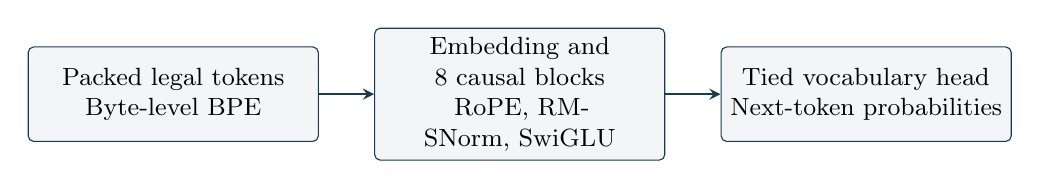
\begin{tikzpicture}[
  cell/.style={draw=inkblue,rounded corners=2pt,fill=inkblue!5,align=center,
    text width=3.45cm,minimum height=12mm,font=\small},
  >={stealth}, every path/.style={draw=inkblue}]
\node[cell] (input) at (0,0) {Packed legal tokens\\Byte-level BPE};
\node[cell] (blocks) at (4.4,0) {Embedding and 8 causal blocks\\RoPE, RMSNorm, SwiGLU};
\node[cell] (output) at (8.8,0) {Tied vocabulary head\\Next-token probabilities};
\draw[->,thick] (input.east) -- (blocks.west);
\draw[->,thick] (blocks.east) -- (output.west);
\end{tikzpicture}
\caption{Phase 1 decoder. The downstream workflows reuse compatible foundation checkpoints.}
\end{figure}


\begin{figure}[H]
\centering
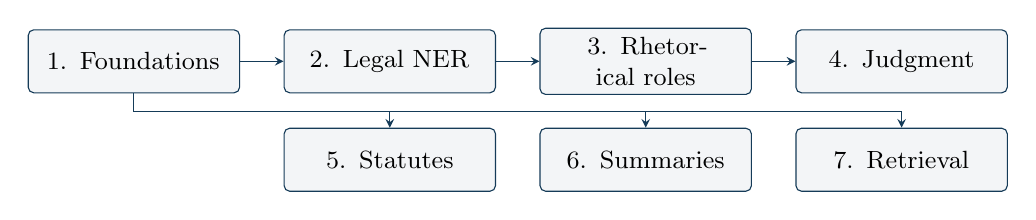
\begin{tikzpicture}[
  task/.style={draw=inkblue,rounded corners=2pt,fill=inkblue!5,
    align=center,text width=2.45cm,minimum height=8mm,font=\small},
  >={stealth}, every path/.style={draw=inkblue}]
\node[task] (p1) at (0,0) {1. Foundations};
\node[task] (p2) at (3.25,0) {2. Legal NER};
\node[task] (p3) at (6.50,0) {3. Rhetorical roles};
\node[task] (p4) at (9.75,0) {4. Judgment};
\node[task] (p5) at (3.25,-1.25) {5. Statutes};
\node[task] (p6) at (6.50,-1.25) {6. Summaries};
\node[task] (p7) at (9.75,-1.25) {7. Retrieval};
\draw[->] (p1) -- (p2);
\draw[->] (p2) -- (p3);
\draw[->] (p3) -- (p4);
\draw (p1.south) -- (0,-.64) -- (9.75,-.64);
\draw[->] (3.25,-.64) -- (p5.north);
\draw[->] (6.50,-.64) -- (p6.north);
\draw[->] (9.75,-.64) -- (p7.north);
\end{tikzpicture}
\caption{Checkpoint initialization across phases. Each downstream workflow trains for its own task.}
\end{figure}

\subsection{Transfer protocol and task heads}

\begin{table}[H]
\centering\small
\caption{Task models linked to the top visible uploads or available workflows.}
\begin{tabularx}{\linewidth}{@{}clY@{}}
\toprule Phase & Initialization & Task model or workflow \\ \midrule
2 & Phase 1 decoder & Bidirectional span boost with BIO and boundary heads. Upload mapping follows the prior report. \\
3 & Phase 2 encoder--decoder & Sentence pooling and contextual Transformer for sequence role prediction. Upload mapping follows the prior report. \\
4 & Phase 3 decoder & Width-48 adapters and a bidirectional GRU over chunks. Upload mapping follows the prior report. \\
5 & Phase 1 decoder & Statute-wise attention, document BiGRU and train-only sparse residual. The extra notebook is the likely match to the generic upload. \\
6 & Phase 1 families & Full suite or fast 04--07 variant. No measured model ranking is available. \\
7 & Phase 1 decoder & Half-depth distilled bi-encoder with lexical/neural fusion. Candidate 07 led the visible submissions. \\
\bottomrule
\end{tabularx}
\end{table}

The Phase 5 upload named \texttt{230437.zip} matches the full-document notebook's logged totals of 13,019 test cases and 57,733 predicted labels. A matching payload hash from Codabench is unavailable. The Phase 4 log records a failure in the optional workspace backup after the seven candidate prediction sets had been produced. The packaged notebook keeps the candidate exports and makes the backup opt-in.

\section{Experiments and Implementation Details}
\subsection{Compute and training protocol}

The saved Kaggle logs show training on two Tesla T4 GPUs with mixed precision. Each workflow records the run configuration, selected checkpoint and prediction files in a phase-specific directory. The fast summarization notebook sets a 20-minute training cap per model and checks it between optimizer updates. Preprocessing, validation and generation sit outside that cap. The runtime figures reported here come from completed logs.

\begin{table}[H]
\centering\small
\caption{Selected configuration settings recorded in the notebooks. Batch units vary by task.}
\begin{tabularx}{\linewidth}{@{}clY@{}}
\toprule Phase & Context and effective batch & Learning rates and budget \\ \midrule
1 & 1,024 tokens / 65,536 tokens per step & Peak $6\times10^{-4}$, 2M token warmup, 200M supervised tokens per foundation. \\
2 & 512 tokens / 32 windows & Backbone $5\times10^{-5}$, head $5\times10^{-4}$ for the base suite. Up to 12 selection epochs with optional refit. \\
3 & 128 tokens per chunk / 4 blocks & Encoder $2\times10^{-5}$, head $2\times10^{-4}$. Up to 6 adaptation epochs. \\
4 & 512 tokens per chunk / 32 cases & Candidate 04 adapter rate $10^{-4}$, head rate $2\times10^{-4}$. Up to 3 adaptation epochs. \\
5 & 384 tokens per chunk / 32 documents & Extra-model encoder $3\times10^{-5}$, head $10^{-3}$, lexical $10^{-2}$. Up to 8 epochs. \\
6 & 1,024 source / 640 target tokens & Fast variant defaults to 16 documents per update and up to 2 epochs. \\
7 & 384 tokens per chunk / 16 queries & Candidate 07 peak $5\times10^{-5}$. Up to 3 student epochs. \\
\bottomrule
\end{tabularx}
\end{table}

\subsection{Local evaluation}

The NER workflow selects checkpoints on held-out documents and requires exact label and character-span matches. The rhetorical-role evaluator checks that the prediction contains one valid label per sentence. In judgment prediction, the supplied-label test run was logged separately from development selection. The extra statute model used one development half to calibrate thresholds and the other to select a checkpoint, then recalibrated on all development cases. The retrieval evaluator checks query coverage and requires seven distinct eligible candidates per query. The generation tasks use reference-based metrics including BERTScore and ROUGE \citep{bertscore,rouge}.

\subsection{Ablations and controlled comparisons}

Two comparisons held the trained model fixed. In Phase 1, the balanced and focused sampling policies used the same decoder and the same 20 held-out prompts. The focused policy raised BLEU-4 from 7.75 to 9.20, while ROUGE-L F1 fell from 0.2172 to 0.2144. The comparison varies a group of decoding settings together. It provides no separate estimate for temperature, truncation or repetition penalty.

On the same 118 Phase 7 queries, candidate 01 scored 0.2446 Micro-F1@7 with its neural ranker alone and 0.2802 with a 0.75 neural weight and BM25. BM25 alone scored 0.2046. The fusion weight was selected on development. The Phase 3 candidates changed both the backbone and the sentence context module, so they compare full configurations.

\section{Results}

\begin{table}[H]
\centering\small
\caption{Phase 1 common-suffix evaluation. Time is the last training invocation.}
\begin{tabular}{@{}lrrrr@{}}
\toprule Architecture & Parameters & Supervised tokens & Perplexity & Hours \\ \midrule
Decoder & 50,340,352 & 200,015,872 & 4.9339 & 1.270 \\
Encoder--decoder & 50,341,888 & 200,001,280 & 5.7232 & 2.747 \\
Local GQA & 50,996,736 & 200,015,872 & 4.9667 & 1.426 \\
Hybrid & 50,348,032 & 200,015,872 & 4.6401 & 1.620 \\
\bottomrule
\end{tabular}
\end{table}

\begin{table}[H]
\centering\small
\caption{Selected local measurements. All-dev calibration uses the same development set for calibration and evaluation.}
\begin{tabularx}{\linewidth}{@{}cYlr@{}}
\toprule Phase & Configuration and split & Metric & Value \\ \midrule
2 & Full decoder, selection epoch 5 & Strict macro-F1 & 0.4720 \\
2 & Bidirectional span boost, validation-tuned & Strict macro-F1 & 0.4730 \\
3 & Full decoder / full encoder--decoder, dev & Macro-F1 & 0.4359 / 0.3888 \\
4 & Decoder adapters, dev / supplied-label test & Macro-F1 & 0.6906 / 0.7025 \\
5 & Full decoder, seven-model suite dev & Macro-F1 & 0.3898 \\
5 & Extra model, selection half / all-dev calibration & Macro-F1 & 0.3920 / 0.4083 \\
7 & BM25 baseline, dev & Micro-F1@7 & 0.2046 \\
7 & LoRMA+ late interaction / distilled student, dev & Micro-F1@7 & 0.2879 / 0.2713 \\
7 & Reciprocal rank fusion ensemble, dev & Micro-F1@7 & 0.2991 \\
\bottomrule
\end{tabularx}
\end{table}

\begin{figure}[H]
\centering
\begin{tikzpicture}
\begin{axis}[width=.47\linewidth,height=4.8cm,
  title={Phase 1 decoder},xlabel={Supervised tokens (millions)},ylabel={Training NLL},
  xmin=0,xmax=200,ymin=0,ymax=11,xtick={0,50,100,150,200},
  grid=major,grid style={gray!20},tick label style={font=\scriptsize},
  label style={font=\small},title style={font=\small}]
\addplot[inkblue,thin,no marks] table[col sep=comma,x=million_tokens,y=train_nll]
  {evidence/phase1_decoder_curve.csv};
\end{axis}
\end{tikzpicture}
\hfill
\begin{tikzpicture}
\begin{axis}[width=.47\linewidth,height=4.8cm,
  title={Phase 5 extra model},xlabel={Epoch},ylabel={Selection-half macro-F1},
  xmin=.75,xmax=7.25,ymin=.365,ymax=.397,xtick={1,2,3,4,5,6,7},
  scaled y ticks=false,ytick={.37,.38,.39},yticklabel style={/pgf/number format/fixed},
  grid=major,grid style={gray!20},tick label style={font=\scriptsize},
  label style={font=\small},title style={font=\small}]
\addplot[tealplot,thick,mark=*] table[col sep=comma,x=epoch,y=selection_half_macro_f1]
  {evidence/phase5_extra_curve.csv};
\end{axis}
\end{tikzpicture}
\caption{Training and checkpoint-selection curves taken from the recorded runs.}
\end{figure}

The extra statute model peaked at epoch 4 on the selection half. Its later score of 0.4083 used thresholds calibrated on all development cases and is reported separately. No comparable Phase 6 score was available. The repository contains the additional variant results and Phase 5 per-label metrics.


\subsection{Models featured in the code package}

Phases 1--4 start with the reported Codabench winner. Two other models are selected by local evaluation because complete per-candidate competition scores are unavailable. Phases 5 and 7 use visible Codabench scores for individual models. The Phase 7 tie at displayed precision is resolved by development Micro-F1@7. Phase 6 code is available for all candidates and the ranking awaits comparable results.

\begin{table}[H]
\centering\small
\caption{Three individual models featured per phase. Phase 6 candidates are unranked.}
\begin{tabularx}{\linewidth}{@{}cYYY@{}}
\toprule Phase & First selection & Second selection & Third selection \\ \midrule
1 & Balanced decoder & Balanced hybrid & Balanced local GQA \\
2 & 08 Bidirectional span boost & 01 Full decoder & 03 Local GQA LoRA \\
3 & 02 Full encoder--decoder & 01 Full decoder & 07 Distilled decoder \\
4 & 04 Decoder adapters & 01 Full decoder & 03 Local GQA LoRMA+ \\
5 & Extra full-document decoder & 02 Partial encoder--decoder & 01 Full decoder \\
6 & 01 Full encoder--decoder & 02 Decoder LoRMA+ & 06 Distilled decoder \\
7 & 07 Distilled decoder & 06 Decoder cross-encoder & 03 Local GQA LoRMA+ \\
\bottomrule
\end{tabularx}
\end{table}

\section{Error Analysis and Discussion}

\subsection{Phase-wise failure modes}

The Phase 1 held-out evaluation contains only 20 prompts and shows that the decoding policies can change metric order. No manual audit of legal claims or citations is recorded. In Phase 2, the full decoder achieved F1 of 0.970 on dates and 0.064 on applicants. The saved error table includes a witness span prediction at offsets 864--869 in one held-out document that did not match a gold span. The exact-match diagnostic alone leaves open whether the error was a boundary mismatch or an incorrect entity assignment.

The full decoder in Phase 3 assigned Dissent to 19 Corporate Law development sentences even though that split contained no gold Dissent examples. It predicted no Issue labels in the same split, which had three gold instances. In Phase 4, the adapter model's supplied-label test run at threshold 0.5 missed 270 of 762 label-1 cases and assigned label 1 to 180 of 755 label-0 cases. The saved confusion matrix does not show where the decisive passage appeared in each judgment.

For Phase 5, statute 84 had 68 development positives. The full decoder recovered 24 of them and assigned the label to 151 documents in total. This produces recall of 0.353, precision of 0.159 and F1 of 0.219. Phase 6 has no verified generated summaries for error review. For Phase 7, the distilled retriever found 244 of 973 annotated relevant pairs in development. Its 826 returned pairs included 582 without relevance annotations. The lexical shortlist retained 61.3\% of annotated relevant pairs on development, placing an upper bound of 0.4936 on Micro-F1@7 for a ranker restricted to that shortlist.

\clearpage
\subsection{What the metrics measure}

BERTScore measures similarity to a reference using contextual representations, while ROUGE measures overlapping text units \citep{bertscore,rouge}. A summary can score well and still misstate a holding. In entity recognition, one incorrect boundary is enough to lose an otherwise plausible match. In retrieval, Micro-F1@7 counts annotated relevance within the seven returned items, with every evaluated query contributing its set of pairs. Those measures serve different tasks and do not measure readiness for legal use.

\subsection{Limitations and follow-up experiments}

The evidence comes from course splits and a two-T4 environment. The small Phase 1 generation sample and Phase 3 domain splits limit comparisons, particularly for labels with little or no development support. The longer workflows trade the amount of text processed against compute. Useful checks would hold the checkpoint fixed and vary the number of judgment chunks or the retrieval shortlist size on a separate split. For summarization, a completed run would support a review that checks each cited authority and holding against the input case.

\subsection{A difference between development and competition results}

The development retrieval ensemble reached 0.2991 Micro-F1@7, ahead of the distilled student's 0.2713. In the available Codabench results, the student recorded 0.2593 and the ensemble 0.2552. The two evaluations therefore give different orders for those systems. This record contains no test labels with which to assign a cause to that reversal.

\section{Conclusion}

The repository contains the implementations used to train four foundations from scratch and the task code for all seven phases. The saved experiments record a common-suffix perplexity of 4.6401 for the hybrid foundation, a strict entity holdout macro-F1 of 0.4720 for the full decoder, and a Codabench Micro-F1@7 of 0.2593 for the distilled retriever. The results cover distinct tasks and splits. Phase 6 is represented by the full and fast notebook variants, with its training and competition outcomes still unverified.

\clearpage
\begin{thebibliography}{9}
\bibitem[CS781 course staff(2026)]{course}
CS781 course staff, \textit{Capstone Document}, Indian Institute of Technology Kanpur, 2026. Official task, data, evaluation, and submission brief.
\bibitem[Vaswani et al.(2017)]{vaswani}
A. Vaswani et al., \emph{Attention Is All You Need}, NeurIPS, 2017.
\bibitem[Su et al.(2021)]{rope}
J. Su et al., \emph{RoFormer: Enhanced Transformer with Rotary Position Embedding}, arXiv:2104.09864, 2021.
\bibitem[Zhang and Sennrich(2019)]{rmsnorm}
B. Zhang and R. Sennrich, \emph{Root Mean Square Layer Normalization}, NeurIPS, 2019.
\bibitem[Shazeer(2020)]{swiglu}
N. Shazeer, \emph{GLU Variants Improve Transformer}, arXiv:2002.05202, 2020.
\bibitem[Zhang et al.(2020)]{bertscore}
T. Zhang, V. Kishore, F. Wu, K. Q. Weinberger, and Y. Artzi, \emph{BERTScore: Evaluating Text Generation with BERT}, ICLR, 2020.
\bibitem[Lin(2004)]{rouge}
C.-Y. Lin, \emph{ROUGE: A Package for Automatic Evaluation of Summaries}, Text Summarization Branches Out, 2004.
\end{thebibliography}



\clearpage
\section*{LLM Usage Declaration}

\textbf{Q1. Which LLMs were used?} The available project history records OpenAI ChatGPT and OpenAI Codex. The exact versions of the models used in earlier chats are unavailable in that record.

\medskip
\textbf{Q2. Where was an LLM used?} This table records uses visible in the project history and in preparation of this report.

\begin{table}[H]
\centering\small
\begin{tabularx}{\linewidth}{@{}p{.34\linewidth}lY@{}}
\toprule Part & Recorded & Purpose \\ \midrule
Understanding concepts or papers & Yes & Explanations of architectures and research. \\
High-level ideation & Yes & Model and workflow alternatives. \\
Debugging ancillary snippets & Yes & Repairs to loading, runtime and export code. \\
Plotting or visualization & Yes & Figures from the saved run metrics. \\
Grammar or writing style & Yes & Revisions to report language. \\
Report structure or wording & Yes & LaTeX, tables and report prose. \\
Model architecture design & Yes & The project chat contains proposed architectures and task heads. \\
Hyperparameter search or tuning & Yes & The chat contains suggested settings and selection logic. The full scope is unverified. \\
Analysis or conclusions & Yes & Codex compiled measured comparisons and prepared the evidence summary and conclusion in this version. \\
Core training or inference code & Yes & Notebook implementation and repairs appear in the project chat. \\
Other & Yes & Code packaging, archive checks and replay of local evaluation. \\
\bottomrule
\end{tabularx}
\end{table}

\textbf{Q3. What other sources were used?} The report draws on the course brief, official course dataset, evaluator scripts and the references cited above. The notebooks and repository also preserve implementation and research references.

\medskip
\textbf{Q4. What was the student's contribution?} The student has not provided a personal contribution statement for this version.

\end{document}
